\begin{frame}{$\chi_b$ yields systematic uncertainties. Unknown $\sigma{\chi_{b2}}/\sigma{\chi_{b1}}$ ratio (1)}

\centering

The $\sigma(\chi_{b2})/\sigma(\chi_{b1})$ ratio prediction:

\resizebox{.5\textwidth}{!}{
\setlength{\unitlength}{1mm}
\begin{picture}(75,60)
%
 \put(0,0){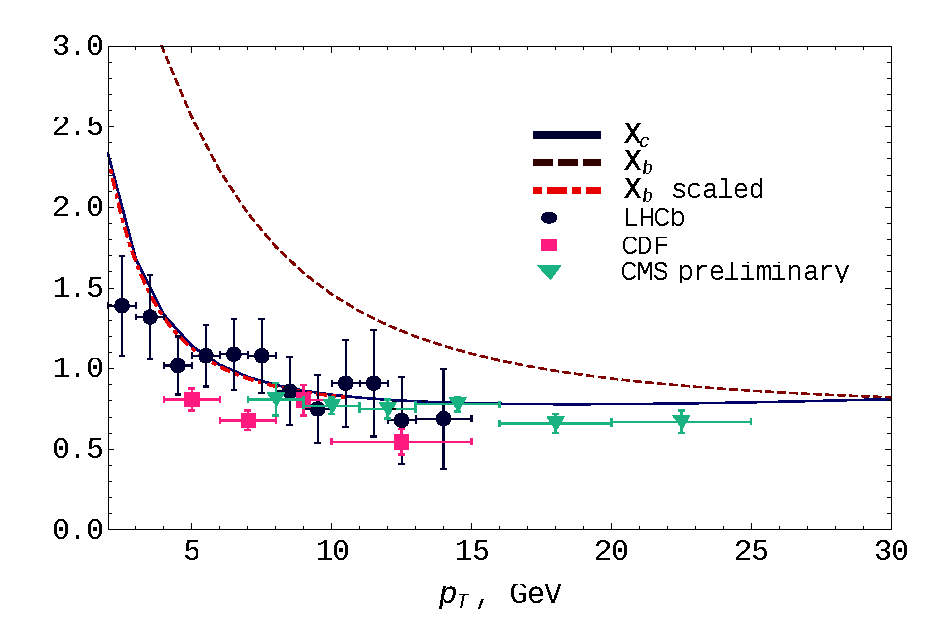
\includegraphics[width=75mm, height=60mm]{theory/ratio}}
 \put(-1,22){\begin{sideways}$\sigma({\chi_2})/\sigma({\chi_1}$)\end{sideways}}
\end{picture}
} 

\footnotesize
Transverse momentum distributions of the
$d\sigma\left[\chi_{2}\right]/d\sigma[\chi_{1}]$ ratio. Solid and dashed lines
stand for charmonium and bottomonium mesons. The dot-dashed line corresponds to
the rescaled bottomonium ratio:
$\sigma_{b2}/\sigma_{b1}(M_{\chi_c}/M_{\chi_b}p_T)$. The experimental results
for charmonium from LHCb are shown with dots, CDF --- with rectangles, and CMS
--- with triangles.
\end{frame}
